% Motivation paragraph
Theoretical motivation
in~\Cref{sec:hh_motivation}.\todo[inline]{Should say something that
  new physics could alter the self-coupling constant.}

In the current experimental environment of HEP, direct searches for
non-resonant Higgs boson pair production are the most sensitive probes
of the Higgs boson self-coupling constant, \lambdahhh, due to the
large sensitivity of the total and differential non-resonant \HH
production cross section to anomalous values of \lambdahhh. Hereafter,
the self-coupling constant is given in terms of the modifier
$\klambda = \lambdahhh / \lambdahhh^{\text{SM}}$ relating an assumed
value of the self-coupling constant to the value predicted by the SM.

The non-resonant \HH production cross section via \ggF and VBF is
shown in \Cref{fig:hh_xsec_incl} as a function of \klambda. The
production via \ggF is the dominant contribution to the total
non-resonant \HH production cross section throughout the considered
\klambda range.
% exceeding cross section of the VBF production mode by at elast a
% factor of about five (18 for SM \HH production).
For the \ggF production mode, the destructive interference between the
box and triangle diagram becomes maximal at about $\klambda = 2.3$ at
which point the cross section reaches a minimum of approximately
\SI{13}{\femto\barn}. Similar behaviour is shown for the VBF
production mode, although involving different diagrams (cf.\
\Cref{fig:hh_feynmans}) and yielding a minimum in cross section below
$\klambda = 2$.

\begin{figure}[htbp]
  \centering

  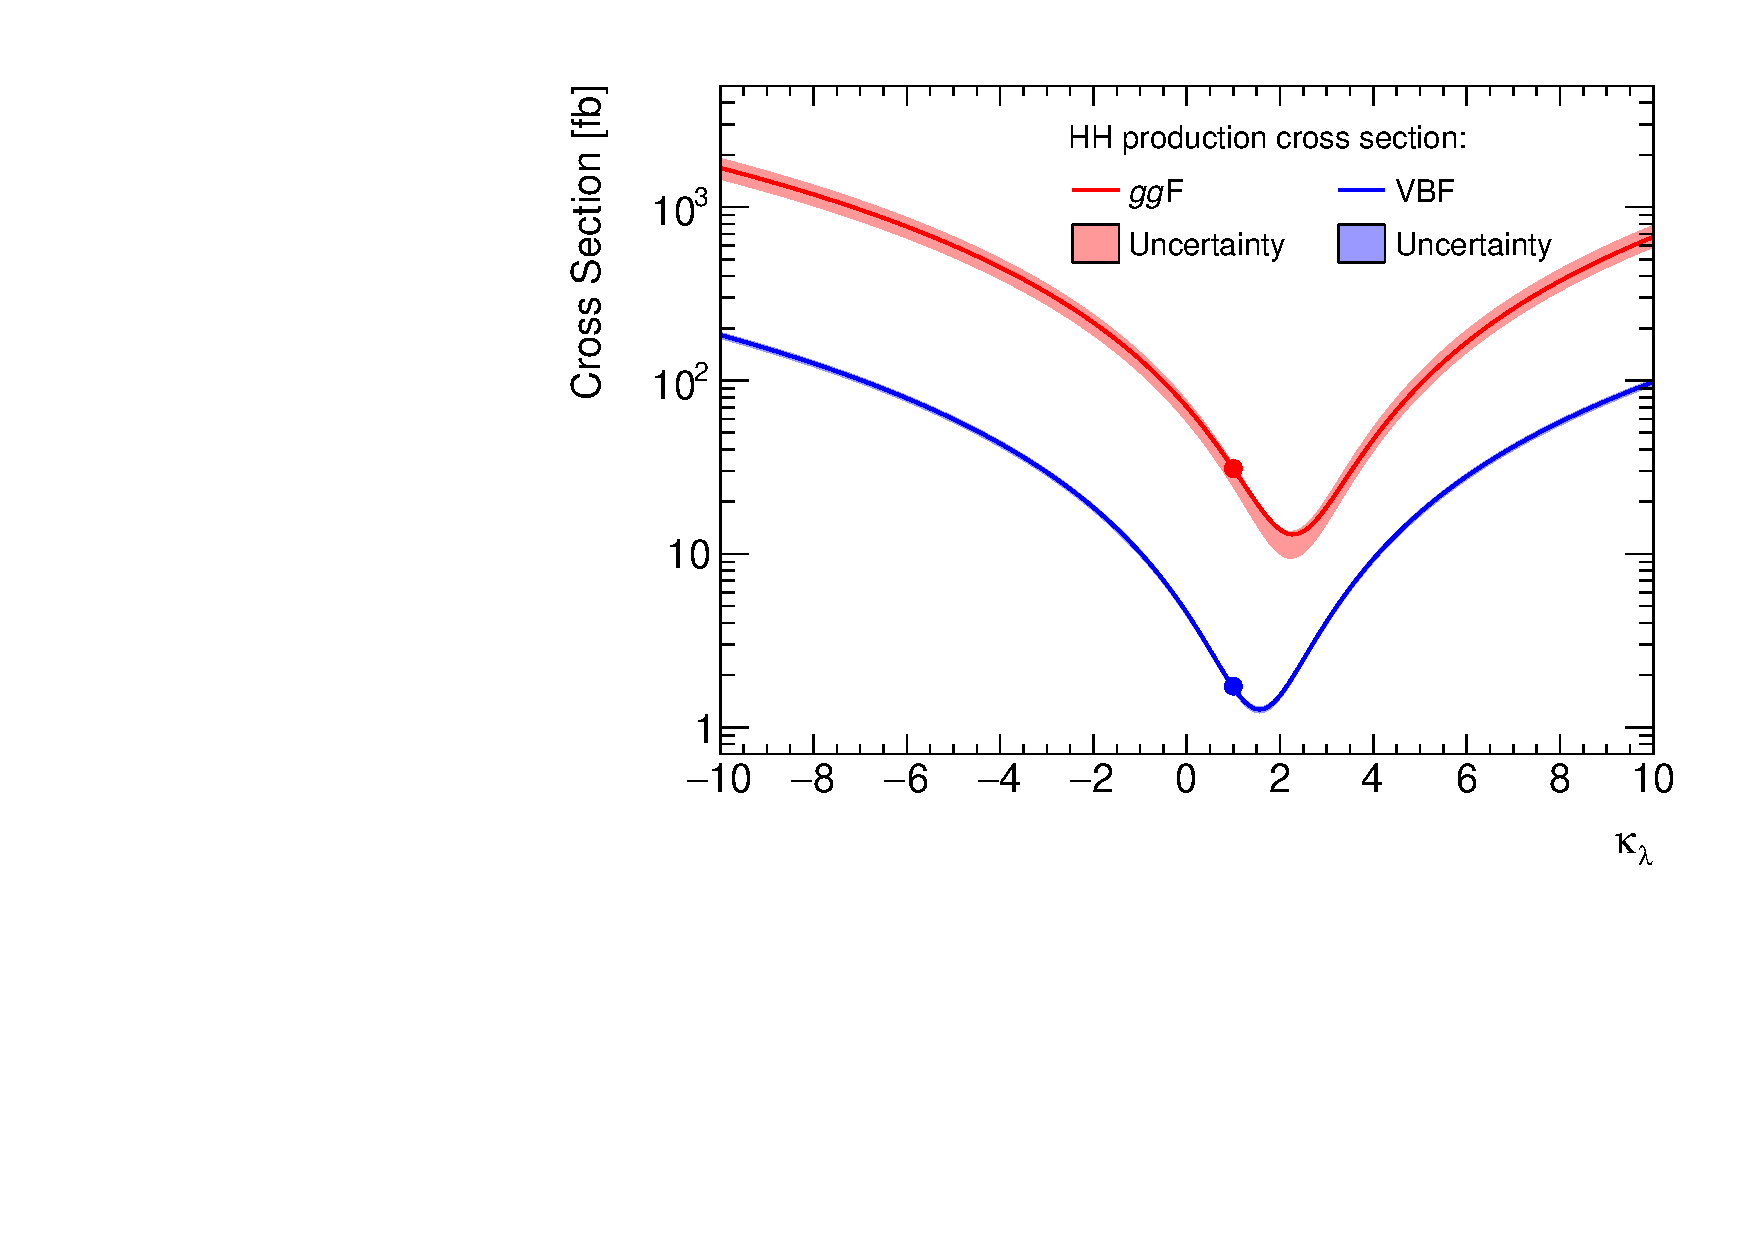
\includegraphics[width=0.55\textwidth]{self_coupling/hh_xsec}

  \caption{\HH production cross section via \ggF and VBF as a function
    of \klambda for $\mH = \SI{125.0}{\GeV}$ in \pp-collisions at
    $\sqrt{s} = \SI{13}{\GeV}$. The production cross section via \ggF
    is given at $\text{NNLO}_{\text{NLO-i}}$ rescaled to
    $\text{NNLO}_{\text{FTapprox}}$ in the $\klambda = 1$
    limit~\cite{Amoroso:2020lgh,Baglio:2020wgt,LHCHWGHH,Grazzini:2018bsd}. The
    production cross section via VBF is obtained from simulation with
    \MGNLO at LO after applying an $\text{N}^3\text{LO}$ $k$-factor
    derived for the SM case~\cite{Dreyer:2018qbw,LHCHWGHH}. The cross
    sections are parameterised as quadratic functions of
    \klambda. Theoretical uncertainties are shown as coloured bands.}%
  \label{fig:hh_xsec_incl}
\end{figure}

In addition to the change in total cross section, anomalous values of
\klambda alter the differential \HH production cross section primarily
in terms of the invariant mass of the pair of Higgs bosons. This is
shown in \Cref{fig:hh_xsec_mhh} for the dominant \ggF production mode
and for five exemplary values of \klambda. The \mHH spectra for
different values of \klambda show large differences in their
\emph{hardness} as measured by the median of the \mHH distribution
in~\Cref{fig:hh_median_mhh}. For \klambda values just below or at the
point of maximum destructive interference between the box and triangle
diagram, the \mHH spectra are moderately hard and have a pronounced
double peak structure. For other values of \klambda, particularly for
$\klambda \approx 3$, the cross section at low \mHH is enhanced
resulting in comparatively soft \mHH spectra.

\begin{figure}[htbp]
  \begin{subfigure}[t]{0.485\textwidth}
    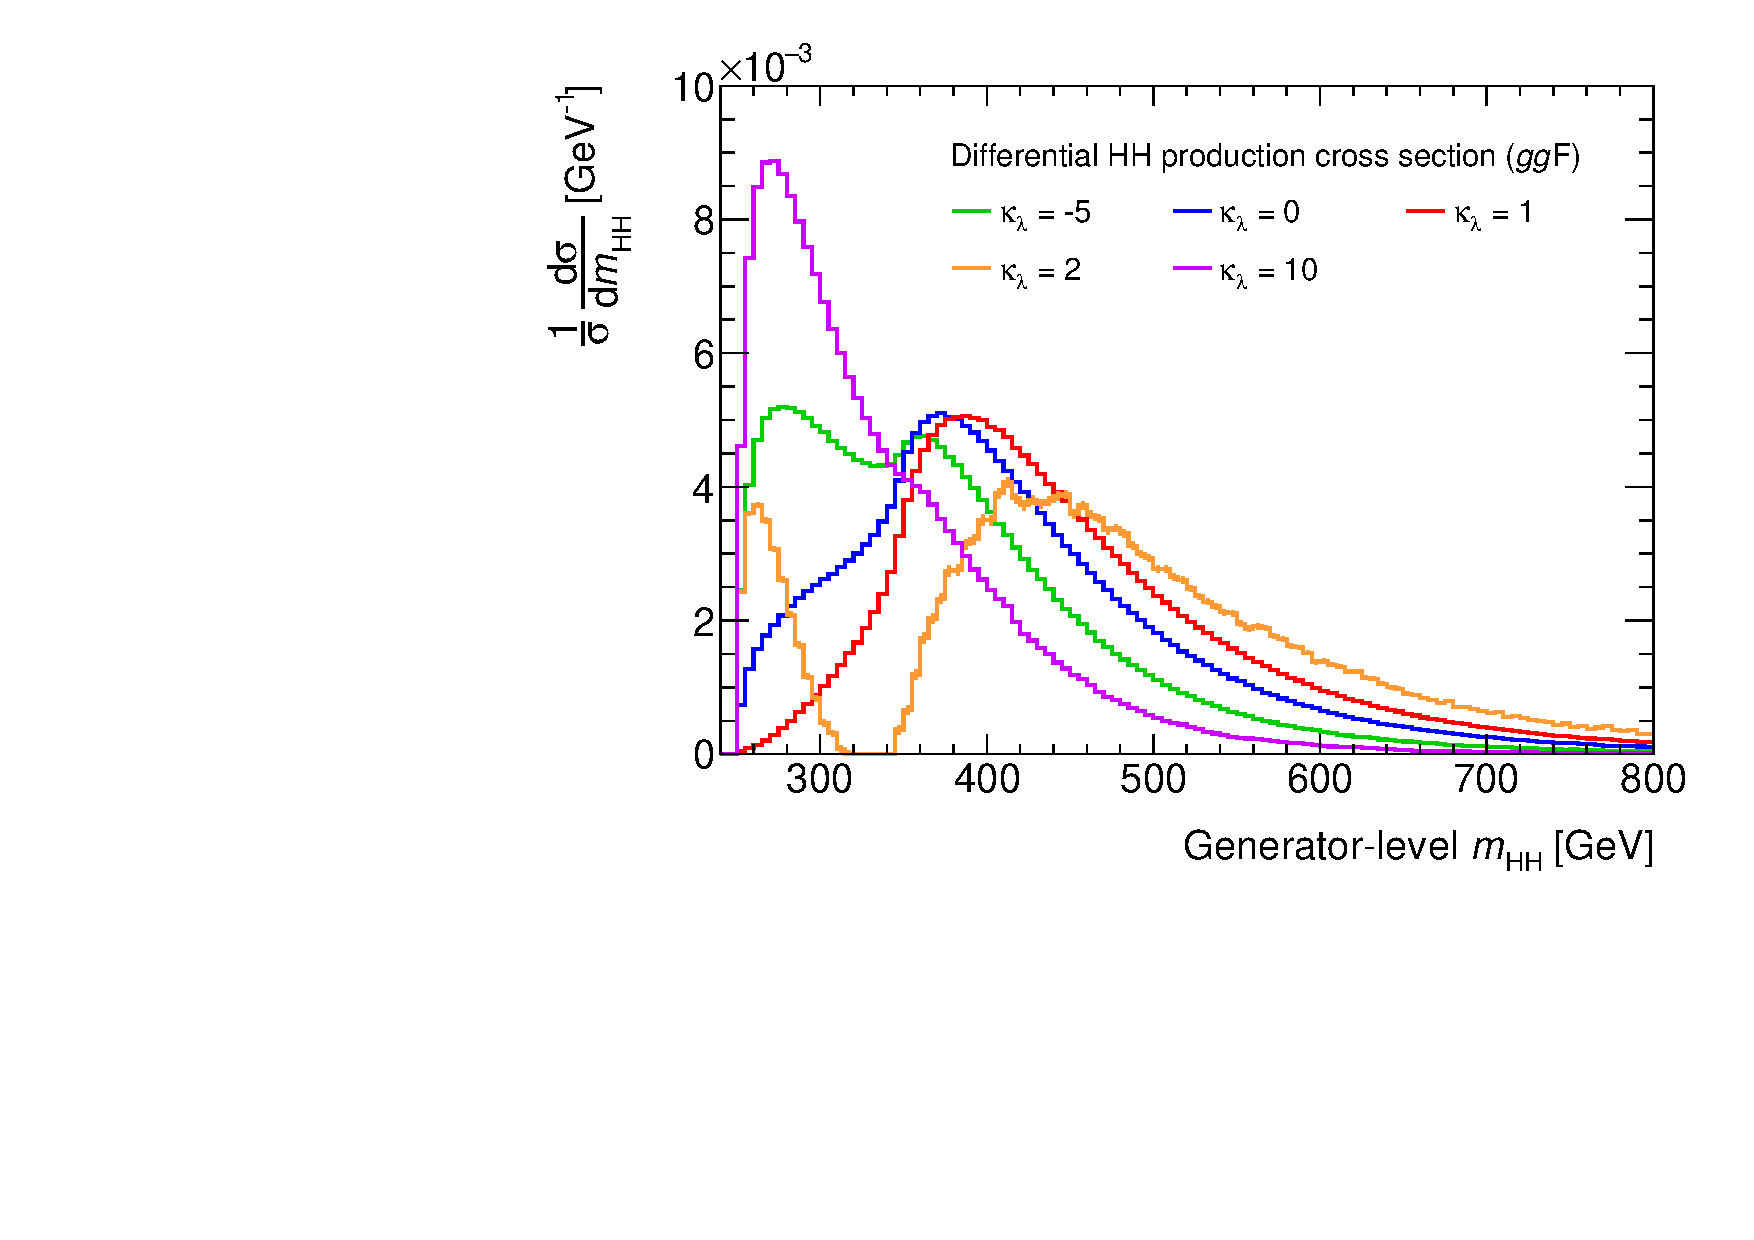
\includegraphics[width=\textwidth]{self_coupling/hh_mhh_vs_klam}
    \subcaption{Differential \HH production cross section with respect
      to \mHH for the \ggF production mode and selected values of
      \klambda. The differential cross sections are normalised by
      dividing by the total cross section. Only statistical
      uncertainties from the finite number of generated events are
      shown.}%
    \label{fig:hh_xsec_mhh}
  \end{subfigure}\hfill%
  \begin{subfigure}[t]{0.485\textwidth}
    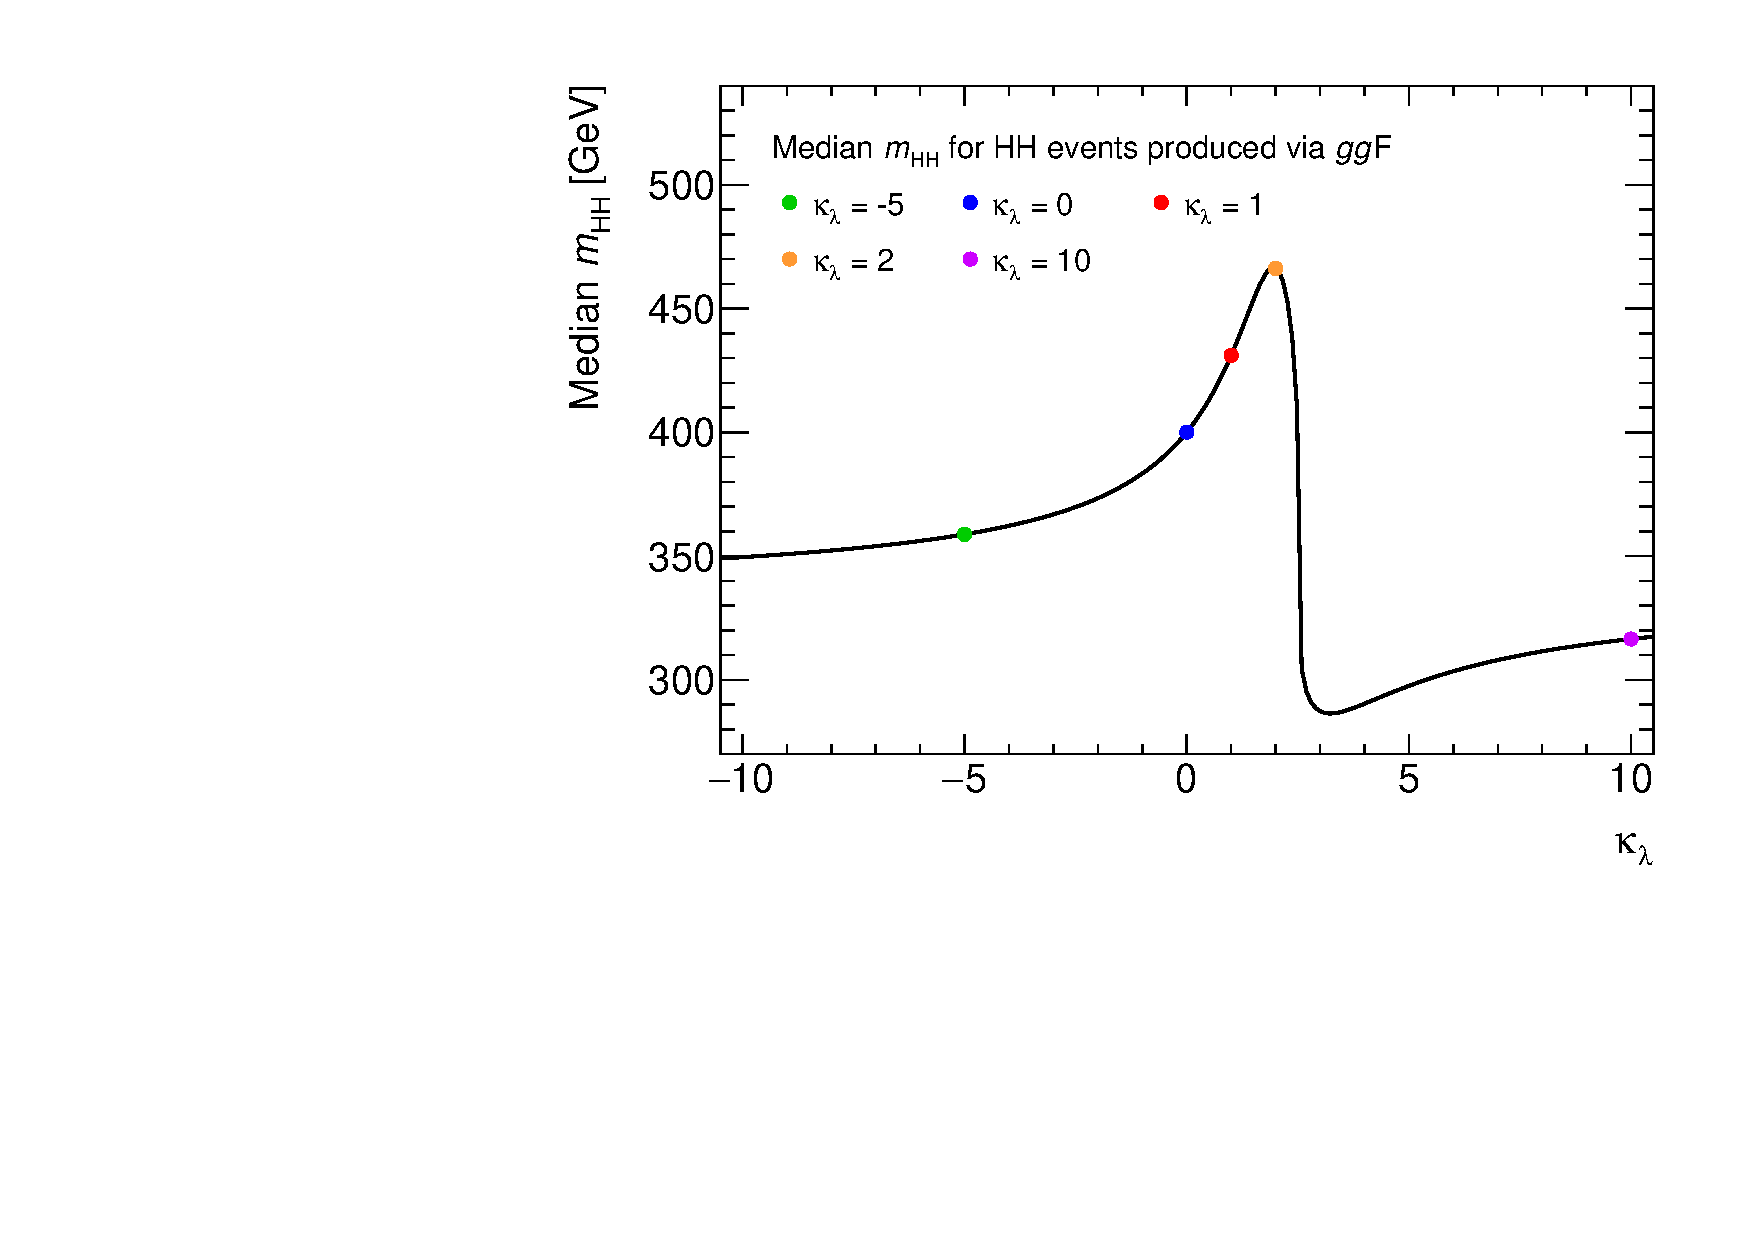
\includegraphics[width=\textwidth]{self_coupling/hh_median_mhh_vs_klam}
    \subcaption{Median value of \mHH for Higgs boson pairs produced
      via \ggF as a function of \klambda.}%
    \label{fig:hh_median_mhh}
  \end{subfigure}

  \caption{Differential cross section of Higgs boson pair production
    via \ggF for selected values of \klambda (a) and the corresponding
    median value of \mHH as a function of \klambda (b). Both are shown
    for \pp-collisions at $\sqrt{s} = \SI{13}{\TeV}$ and assuming
    $\mH= \SI{125.0}{\GeV}$. The cross sections are obtained from
    simulation with \POWHEGBOX[v2] at NLO including the top-quark mass
    dependence~\cite{Heinrich:2019bkc,Heinrich:2020ckp} for
    $\klambda = 0, 1, 10$. Differential cross sections for other
    values of \klambda are estimated using morphing techniques derived
    at LO~\cite{ATL-PHYS-PUB-2019-007}.}
\end{figure}

This chapter presents a reinterpretation of the search for SM \HH
production ($\klambda = 1$) presented in~\Cref{sec:dihiggs} in terms
of non-resonant \HH production with anomalous values of the Higgs
boson self-coupling constant. A reinterpretation of this search yields
constraints on the allowed values of \klambda as the expected number
of signal events in the signal regions is sensitive to the value of
the self-coupling constant. This sensitivity is due to the \klambda
dependency of both the non-resonant \HH production cross section, and
of the signal acceptance of the selections applied in the analysis
which is closely tied to the characteristic \mHH spectrum of a given
\klambda hypothesis.

Previous constraints on \klambda were set by the ATLAS collaboration
using up to \SI{36.1}{\per\femto\barn} of \pp-collision data taken
during Run~2 of the LHC by combining the results of six searches for
non-resonant \HH production. This combination yielded an allowed range
of $-5.0 < \klambda < 12.0$ at \SI{95}{\percent}
CL~\cite{HDBS-2018-58}. The results presented in this chapter are
based on Ref.~\cite{ATLAS-CONF-2021-052} and focuses on the
reinterpretation of the result obtained in \Cref{sec:dihiggs} in the
$\bbbar\tautau$ channel with \SI{139}{\per\femto\barn} of
\pp-collision data.

% These results were superseded by a combination of the most sensitive
% search channels for non-resonant \HH and single Higgs boson
% production by the ATLAS collaboration in
% Ref.~\cite{ATLAS-CONF-2022-050}, which is not discussed in detail in
% this chapter.

This chapter is structured as follows. \Cref{sec:reinterpretation}
describes the statistical model used for the reinterpretation
including its assumptions and limitations. The resulting constraints
on \klambda are presented in \Cref{sec:reinterpretation_results} and
discussed. The chapter concludes
in~\Cref{sec:reinterpretation_conclusion} with an outlook.


\section{Reinterpretation of the Search for SM \HH Production}%
\label{sec:reinterpretation}

The reinterpretation of the search for SM \HH production
($\klambda = 1$) in terms of anomalous values of \klambda is performed
based on the statistical model developed in
\Cref{sec:statistical_analysis}. With respect to the SM \HH search
presented previously, only the signal model used for the statistical
interpretation is altered. The discriminants entering the fit and
their binning remain at the configuration optimised for the SM \HH
signal.

The SM \HH signal model used for the statistical interpretation is
replaced by a model of non-resonant \HH production with arbitrary but
fixed \klambda. Both the \ggF and the VBF production mode are
considered. This signal is normalised according to a cross section of
$\sigma_{HH}^{\klambda}$ which is considered as a POI in the
statistical analysis. Upper limits are set on $\sigma_{HH}^{\klambda}$
as a function of \klambda and compare to the theoretical cross section
for a given value of \klambda. Intervals of \klambda are excluded if
the cross section predicted by theory is larger than the
experimentally determined upper limit.

This reinterpretation makes the assumption that the background model
remains unchanged for different assumed values of \klambda. However,
this is not the case since single Higgs boson production is a small
but non-negligible background and both the production cross sections
and the branching ratios of the Higgs boson decay depend on \klambda.

References on H sensitivity to
\klambda~\cite{ATL-PHYS-PUB-2019-009,Degrassi:2016wml,Maltoni:2017ims}.

In the \klambda range (-3 to 12 based on old results) relevant for
this search change in H->bb or H->tautau branching ratio is below
5\%. This is also not considered for the Higgs decay in signal
processes.

Production cross sections for all except ttH below 10\%. ttH can
change up to 15\%.

- Assuming all other couplings are at their SM value.

- Single Higgs boson production is affected by \klambda only from
higher order EW corrections


\subsection{Signal Model}

\Cref{sec:data_and_simulation}

ggF: Re-weighting

VBF: Linear combination

\todo[inline]{Hadhad channel: Acceptance times efficiency vs mHH.}

\todo[inline]{Hadhad channel: Acceptance times efficiency vs kLambda.}

Should say that bbtautau is only good because the SM is already pretty
hard. -> acceptance vs mHH in \hadhad.


Signal modelling uncertainties:
- Uncertainties from the re-weighting procedure are included
- The signal modelling uncertainties are included


\section{Results}%
\label{sec:reinterpretation_results}


\begin{figure}[htbp]
  \centering

  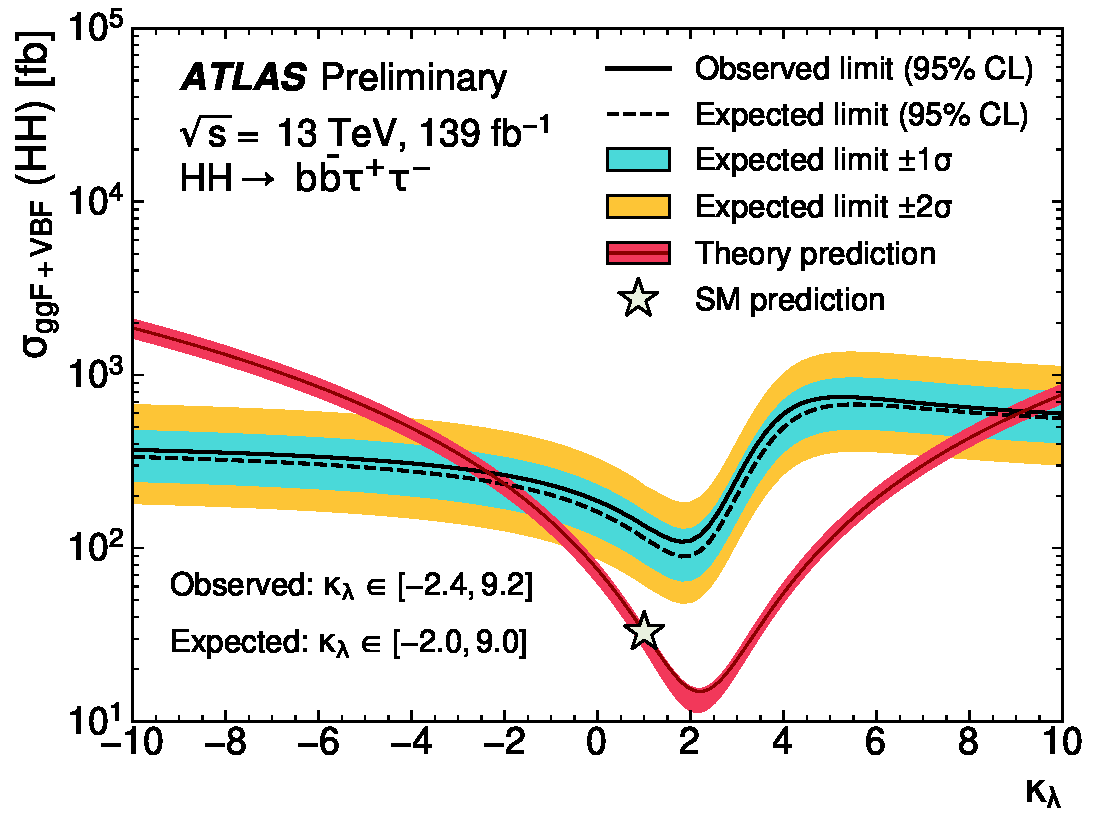
\includegraphics[width=0.6\textwidth]{self_coupling/klam_scan_result}

  \caption{Klambda scan. The figure is taken from
    Ref.~\cite{ATLAS-CONF-2021-052}.}%
  \label{fig:klambda_scan}
\end{figure}


\section{Conclusion and Outlook}%
\label{sec:reinterpretation_conclusion}


The total Higgs boson pair production cross section with anomalous
couplings. Following recommendations by the LHC Higgs Working
Group~\cite{LHCHWGHH}:
\begin{description}

\item[\ggF production mode] The cross sections of \HH production with
  anomalous self-couplings were calculated in
  Ref.~\cite{Amoroso:2020lgh} at $\text{NNLO}_{\text{NLO-i}}$
  (NLO-improved). This prediction is obtained from combining the
  result with the full top-quark mass dependence at
  NLO~\cite{Buchalla:2018yce}


  with NNLO corrections in the $m_{t} \to \infty$
  limit~\cite{deFlorian:2017qfk}.

  Additionally, the prediction is rescaled such that it coincides with
  the SM \HH cross section at $\text{NNLO}_{\text{FTapprox}}$ at
  $\klambda = 1$.

  The total \HH production cross section via \ggF was found to depend
  quadratically on \klambda and is thus parameterised
  accordingly~\cite{LHCHWGHH}.

\item[VBF production mode]

\end{description}


\todo[inline]{Read YR about Higgs cross section predictions:
  \url{https://cds.cern.ch/record/2227475/files/CERN-2017-002-M.pdf}}

Sample combination method:~\cite{ATL-PHYS-PUB-2019-007}


\todo{Updated result from H+HH
  combination~\cite{ATLAS-CONF-2022-050}.}


%%% Local Variables:
%%% mode: latex
%%% TeX-master: "../../phd_thesis"
%%% End:
